% Compile from this folder with pdfLaTeX, BibTeX, then pdfLaTeX twice.
\documentclass[10pt,a4paper]{article}
\usepackage[margin=1.65cm]{geometry}
\usepackage[T1]{fontenc}
\usepackage[utf8]{inputenc}
\usepackage{graphicx,booktabs,array,float}
\usepackage[font=small,labelfont=bf]{caption}
\usepackage[numbers]{natbib}
\usepackage{titlesec}
\usepackage[colorlinks=true,urlcolor=blue,linkcolor=black,citecolor=black]{hyperref}
\setlength{\parindent}{0pt}
\setlength{\parskip}{4pt}
\setlength{\textfloatsep}{6pt}
\setlength{\intextsep}{6pt}
\setlength{\abovecaptionskip}{4pt}
\titleformat{\section}{\large\bfseries}{\thesection.}{0.4em}{}
\titleformat{\subsection}{\normalsize\bfseries}{\thesubsection}{0.4em}{}
\titlespacing*{\section}{0pt}{6pt}{3pt}
\titlespacing*{\subsection}{0pt}{6pt}{3pt}
\renewcommand{\arraystretch}{1.04}
\graphicspath{{figures/}}
\begin{document}
\begin{center}
{\Large\bfseries SENTINEL: Network Traffic Analysis}\\[2pt]
{\small DPA Part 1 -- Volume (Spark SQL), Fall 2026 -- Universit\'e Claude Bernard Lyon 1}\\[2pt]
Waleed Mahmood, Shiza Noor, Yasmine Bourbon\\[2pt]
{\small\href{https://github.com/waleedm96/DPA-Cybersecurity-Analysis}{github.com/waleedm96/DPA-Cybersecurity-Analysis} -- Review draft, 17 October 2026}
\end{center}
\vspace{-5pt}

\section{Questions}
The overarching question is: how can network traffic analysis distinguish attacks from normal activity, detect suspicious patterns as traffic arrives, and identify important hosts in attacks? This report covers batch analysis only. Its two questions are:
\textbf{(1)} What traffic patterns distinguish normal activity from attacks?
\textbf{(2)} Which network services and traffic characteristics are associated with different attack categories?

\section{Data and integration}
\begin{center}\small
\begin{tabular}{@{}llll@{}}
\toprule
Source & Raw CSV size & Raw records & Licence / terms \\
\midrule
Original CSE-CIC-IDS2018 \cite{dataset1} & 6.89 GB (10 files) & 16,233,002 & Redistribution with citation + AWS link \\
IANA service/port registry \cite{dataset2} & About 1.15 MB & 14,536 & CC0 1.0 \\
\bottomrule
\end{tabular}
\end{center}
The original traffic release covers ten collection days between 14 February and 2 March 2018. Nine files have 80 columns; 20 February has 84. A flow record summarises packets exchanged between endpoints; it is not one packet or one user.

A broadcast left join matches destination port and protocol (6 = TCP, 17 = UDP). Combining IANA aliases first keeps one lookup row per key and preserves all 15,727,874 cleaned traffic rows. Unmatched rows stay; no match does not prove a port is unregistered or malicious.

Spark processes the large, wide tables in partitions using two local worker threads. Parquet lets later queries read only needed columns, reducing the memory and reading costs of repeated laptop analysis.

\section{Pipeline}
\begin{center}\small
\fbox{\shortstack{Traffic + IANA\\CSV files}} $\rightarrow$
\fbox{\shortstack{Explicit schemas\\Raw Parquet}} $\rightarrow$
\fbox{\shortstack{Cleaning\\Audit counts}} $\rightarrow$
\fbox{\shortstack{Broadcast\\left join}} $\rightarrow$
\fbox{\shortstack{Spark summaries\\Tables + charts}}
\end{center}
Check headers and 500 rows per file, then process the selected dataset. DataFrame filters, aggregation, and window ranking calculate category and service summaries. Only small result tables enter Python for plotting.

\section{Cleaning and row counts}
Traffic changes from \textbf{16,233,002 to 15,727,874 rows}: 505,128 rows removed (3.11\%). IANA changes from \textbf{14,536 to 11,391 lookup rows}. The table lists sequential removals and changes; excluded valid entries and merged aliases are distinguished from dirty rows.
\begin{center}\small
\begin{tabular}{@{}lrr@{}}
\toprule
Step & Traffic: removed / changed & IANA: removed / changed \\
\midrule
Malformed CSV records & 59 / 0 & 0 / 0 \\
Duplicate complete records & 410,707 / 0 & 0 / 0 \\
Missing required values (including numeric NaN) & 58,343 / 0 & 2,813 / 0 \\
Infinite measurements & 36,005 / 0 & --- \\
Impossible measurements / port values & 14 / 0 & 0 / 0 \\
Parse dates and check collection period & 0 / 15,727,874 & --- \\
Valid entries outside individual TCP/UDP scope & --- & 100 / 11,623 \\
Combine service aliases per port/protocol & --- & 232 / 226 \\
\bottomrule
\end{tabular}
\end{center}
Drop required missing values rather than guess. An unnamed IANA entry can be valid but cannot label a service. Deduplicate all typed source fields within each traffic file. Remove negative measurements, invalid codes, and bytes without packets; keep large finite values. Dates use day/month/year. Text normalisation and IANA format checks change/remove zero rows. Reject reversed IANA ranges and ports outside 0--65535. Alias merging changes 226 keys. The audit saves every step's counts.

\section{Main design decisions}
Use explicit integers for ports, long integers for counts, doubles for measurements, and text for dates until cleaning. IANA ports start as text to keep ranges. Keep 11 traffic fields plus filename and three IANA lookup fields; raw tables retain all columns. Missing IP fields in nine files are expected and unused. Analyse all 15 labels. \textbf{Results below use full data; the subset only supports quick evaluation.}

\newpage
\section{Results: answers to the two questions}
\subsection*{Question 1 -- How does attack traffic differ from normal activity?}
There are \textbf{13,374,907 normal records (85.04\%)} and \textbf{2,352,967 attack records (14.96\%)}. Categories are identified by the supplied labels; the analysis compares these known groups rather than predicting an unknown record's label.

\textbf{Recorded bytes per packet} divides the category's total recorded bytes (both directions) by its total packets. \textbf{Median packets/s} is the approximate middle of its supplied \texttt{Flow Pkts/s} rates: about half the records lie below it and half above. This is the rate \emph{within a flow record}, not whole-network traffic per second.

\begin{table}[H]\centering\small
\caption{Full-data results for every label. Display names are shortened; source labels are unchanged.}
\begin{tabular}{@{}lrrr@{}}
\toprule
Category & Records & \shortstack{Recorded bytes\\per packet} & \shortstack{Median packets/s\\within a record} \\
\midrule
Normal (Benign) & 13,374,907 & 459.02 & 103.73 \\
DDoS HOIC & 668,461 & 93.75 & 474.95 \\
DDoS LOIC-HTTP & 576,191 & 34.20 & 3.83 \\
DoS Hulk & 434,873 & 30.69 & 145.55 \\
Bot & 282,310 & 49.68 & 776.74 \\
Infilteration & 160,604 & 264.32 & 1,715.27 \\
SSH brute force & 117,322 & 103.95 & 120.98 \\
DoS GoldenEye & 41,455 & 150.51 & 1.04 \\
FTP brute force & 39,346 & 0.00 & 400,000.00 \\
DoS SlowHTTPTest & 19,462 & 0.00 & 333,333.33 \\
DoS Slowloris & 10,285 & 116.46 & 0.17 \\
DDoS LOIC-UDP & 1,730 & 32.00 & 1,016.04 \\
Web brute force & 611 & 479.22 & 4.50 \\
XSS brute force & 230 & 794.45 & 5.74 \\
SQL Injection & 87 & 315.69 & 1.73 \\
\bottomrule
\end{tabular}
\end{table}

\begin{figure}[H]\centering
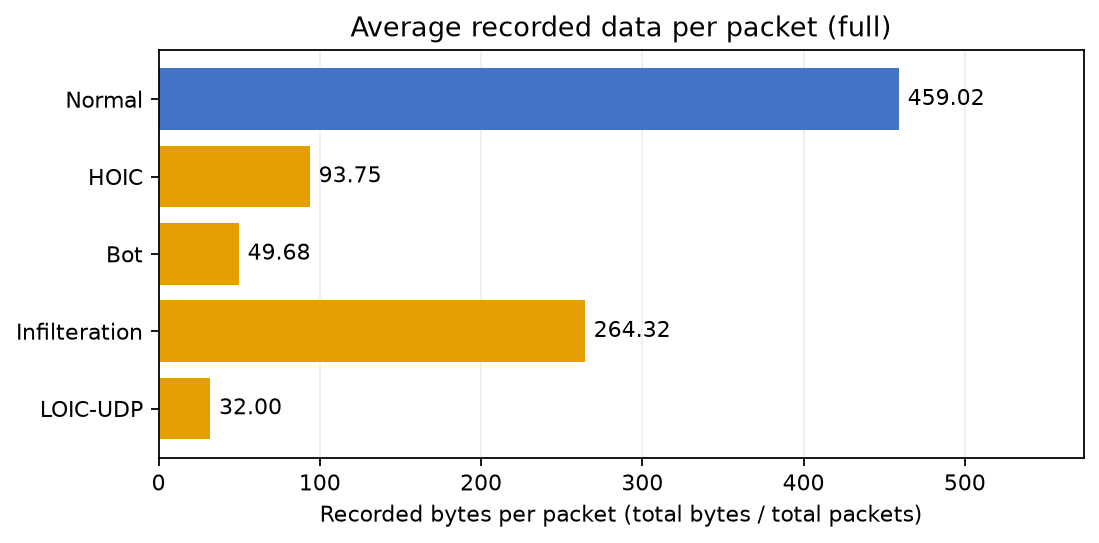
\includegraphics[width=0.76\linewidth]{bytes_per_packet.png}
\caption{Five categories shown for readability. The table above includes all 15 labels; no category is removed from the full analysis.}
\end{figure}

\textbf{Answer.} Several attack categories combine smaller recorded data sizes with higher typical packet rates. For example, normal traffic records 459.02 bytes per packet and a middle rate of 103.73 packets/s. HOIC records 93.75 bytes per packet and 474.95 packets/s; Bot records 49.68 and 776.74. Across all attacks pooled, the corresponding values are 35.53 bytes per packet and 166.82 packets/s. These are measured differences between the labelled groups in this dataset.

\textbf{No universal ``higher means attack'' rule follows.} Slowloris has a lower middle rate (0.17 packets/s), while XSS has more recorded bytes per packet than normal. FTP brute force and SlowHTTPTest show zero recorded bytes and very high rates; counters and short durations require caution. Group differences do not establish that individual values never overlap. This is descriptive analysis, not a proven detector.

\newpage
\subsection*{Question 2 -- Which services and traffic characteristics are associated with attacks?}
\textbf{Answer.} Services are associated with particular labels: FTP brute force sends 100\% of records to 21/TCP, SSH brute force 99.99\% to 22/TCP, Bot 98.39\% to 8080/TCP, and HOIC 100\% to 80/TCP. Normal traffic is more spread out: 30.06\% on 53/UDP, 14.92\% on 443/TCP, and 12.55\% on 80/TCP.

\begin{figure}[H]\centering
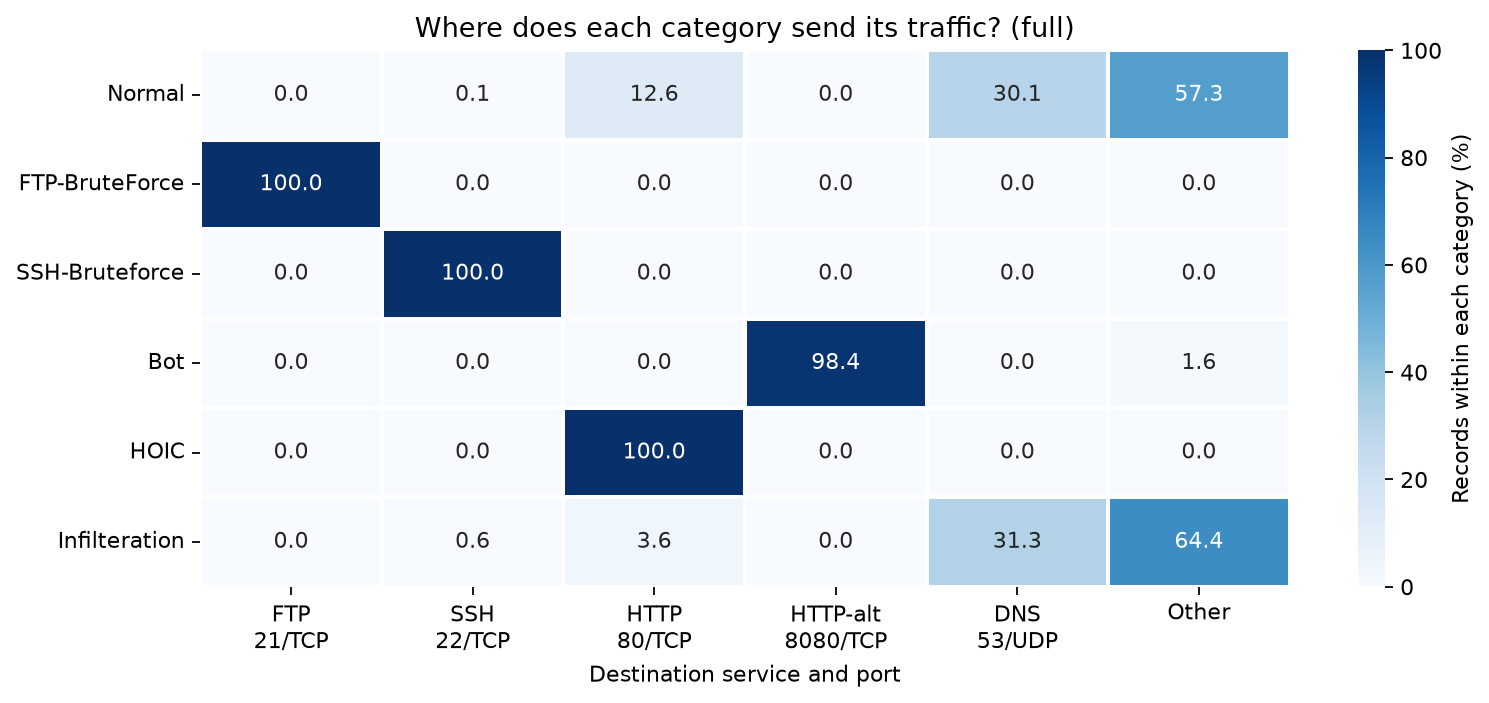
\includegraphics[width=0.91\linewidth]{attack_services.png}
\caption{Percent of each category's records sent to five selected port/protocol pairs. ``Other'' contains all remaining pairs, including registered ports. Values are rounded to one decimal place, so small nonzero shares can appear as 0.0.}
\end{figure}

An \textbf{active minute} is a source-file minute with at least one record for that label and service. Dividing records by active minutes measures activity on that service. It counts flow records, not packets or unique connections, and differs from Question 1's packet rate.

\begin{table}[H]\centering\small
\caption{Full-data service concentration and mean records per active minute. Normal and attack groups have their own active minutes, not matched observation windows.}
\begin{tabular}{@{}llrrr@{}}
\toprule
Attack category & Destination & \shortstack{Attack records\\on this pair (\%)} & \shortstack{Normal\\records/min} & \shortstack{Attack\\records/min} \\
\midrule
FTP brute force & FTP (21/TCP) & 100.00 & 1.32 & 401.49 \\
SSH brute force & SSH (22/TCP) & 99.99 & 3.90 & 1,275.16 \\
Bot & HTTP-alt (8080/TCP) & 98.39 & 1.70 & 812.14 \\
HOIC & HTTP (80/TCP) & 100.00 & 382.80 & 29,063.52 \\
\bottomrule
\end{tabular}
\end{table}

HOIC has 668,461 records on 80/TCP in 23 active minutes; normal traffic has 1,678,562 in 4,385 active minutes: about 29,064 versus 383 records/min. This shows concentration and intensity in the experiment, but the different periods prevent a controlled comparison. Slowloris has only 239.19 records/min on 80/TCP, below normal.

All remaining labels were analysed. Hulk, GoldenEye, and Slowloris use 80/TCP exclusively; LOIC-HTTP uses it for 99.86\%. Web brute force, XSS, and SQL injection use it for 75.29\%, 97.83\%, and 100\%. LOIC-UDP uses 80/UDP (``Other''). Infilteration is spread out (31.30\% on 53/UDP, 18.20\% on 443/TCP). SlowHTTPTest appears on 21/TCP; this unexpected association is reported without relabelling.

\subsection*{Limits and reproduction}
Registered ports do not verify the application or prove safety \cite{dataset2}; this IANA snapshot is not the 2018 registry. Experimental labels, counters, different periods, and unequal category sizes limit generalisation (SQL injection has only 87 records). Part 1 evaluates no detector, streaming system, or host graph.

Follow the repository README and run the notebook in Docker with \texttt{USE\_SUBSET = False} for full results. The default subset is for quick evaluation and has different proportions. Source CSVs stay unchanged; \texttt{reports/} contains cleaning counts, all-label results, and four full-data charts.

\begingroup\small
\setlength{\bibsep}{2pt}
\bibliographystyle{plainnat}
\bibliography{references}
\endgroup
\end{document}
